\section{Experiments}\label{sec:experiments}

All numbers in this section are produced by the scripts in \repo{code/experiments} and are reported in the summary files of \repo{results}; the tables below are generated from those files by \repo{code/experiments/make_tables.py}. Every reported bound includes a charge for the codec designs we tried on the same data during development (4 bits per description, and the disagreement term at confidence $\delta_2/16$; \repo{code/experiments/accounting.py}).

\subsection{Boolean tasks with a known input distribution}\label{sec:exp-bool}

\paragraph{Setup.} Inputs are uniform on $\{\pm1\}^{50}$. Targets: the parity of 3 fixed coordinates (\texttt{parity3}), the majority of 5 (\texttt{maj5}), the AND of 3 (\texttt{and3}), a random truth table on 6 coordinates (\texttt{junta6}), and the majority of all 50 (\texttt{fullmaj}), plus \texttt{maj5} and \texttt{parity3} with 10\% of the training labels flipped. The network $f$ is an MLP of widths $(50,512,512,1)$ with 289{,}281 parameters, trained with Adam (learning rate $10^{-3}$, batch 64) until it reaches zero training error and a mean training loss below $0.01$. We use $m\in\{250,\dots,16000\}$ and three seeds per setting (training set and initialization). The bound is \cref{thm:reduction} with the codec of \cref{sec:methods}; the disagreement term uses $2\times10^5$ fresh uniform inputs.

\paragraph{Results.} \Cref{fig:boolean,tab:boolean} show the main finding: wherever $f$ generalizes, the bound on $f$ is close to its test error. Across the learning curve the bound is roughly test error plus $L\ln2/m$, where $L$ is 28--100 bits (a truth table on the relevant coordinates or a linear threshold function). The parameter-counting baseline (32 bits per parameter, about $9.3\times10^6$ bits) and the VC baseline are 1.0 for every network. Where $f$ has not learned the target (\texttt{parity3} at $m\le1000$), the bound is vacuous, correctly. Where $f$ has partially learned it, the bound still tracks: at $m=2000$, \texttt{parity3} networks have test error $0.29$ and bound $0.30$. The best $g$ is then the true parity, with zero training errors, and $\Pr[f\ne g]$ is $f$'s error.

\paragraph{Interpolating noisy labels.} With 10\% label noise, $f$ fits every flipped label (zero training error). Its test error on noisy labels is $0.1+0.8\,\Pr[f\ne\text{target}]$. The compressed $g$ is the clean rule, so $\err(g)\approx0.1$ and $\Pr[f\ne g]$ measures the damage done by memorization. At $m=16000$ the bounds are 0.17 against a test error of 0.14 for both tasks. A bound of this kind needs only that $f$ is close to a short program on most of the input space; it does not need $f$ to be simple.

\begin{table}[t]
\centering\small
\begin{tabular}{l r r r r}
\toprule
task & $m$ & test err.\ $f$ & bound on $f$ & bits of $g$ \\
\midrule
\texttt{and3} & 500 & 0.0366 & 0.0875 & 32 \\
\texttt{and3} & 1000 & 0.0056 & 0.0312 & 32 \\
\texttt{and3} & 2000 & 0.0000 & 0.0128 & 32 \\
\texttt{and3} & 4000 & 0.0000 & 0.0064 & 32 \\
\texttt{and3} & 16000 & 0.0000 & 0.0016 & 32 \\
\addlinespace[2pt]
\texttt{fullmaj} & 500 & 0.0656 & 0.2609 & 103 \\
\texttt{fullmaj} & 1000 & 0.0386 & 0.1056 & 77 \\
\texttt{fullmaj} & 2000 & 0.0272 & 0.0688 & 94 \\
\texttt{fullmaj} & 4000 & 0.0148 & 0.0267 & 60 \\
\texttt{fullmaj} & 16000 & 0.0011 & 0.0037 & 48 \\
\addlinespace[2pt]
\texttt{junta6} & 500 & 0.4005 & 0.9364 & 61 \\
\texttt{junta6} & 1000 & 0.3111 & 0.6451 & 78 \\
\texttt{junta6} & 2000 & 0.1685 & 0.3422 & 102 \\
\texttt{junta6} & 4000 & 0.0223 & 0.0418 & 102 \\
\texttt{junta6} & 16000 & 0.0000 & 0.0047 & 102 \\
\addlinespace[2pt]
\texttt{maj5} & 500 & 0.0109 & 0.0910 & 54 \\
\texttt{maj5} & 1000 & 0.0002 & 0.0373 & 49 \\
\texttt{maj5} & 2000 & 0.0001 & 0.0188 & 49 \\
\texttt{maj5} & 4000 & 0.0000 & 0.0095 & 49 \\
\texttt{maj5} & 16000 & 0.0000 & 0.0024 & 49 \\
\addlinespace[2pt]
\texttt{parity3} & 500 & 0.4982 & 0.9695 & 87 \\
\texttt{parity3} & 1000 & 0.4964 & 1.0000 & 225 \\
\texttt{parity3} & 2000 & 0.2876 & 0.3043 & 35 \\
\texttt{parity3} & 4000 & 0.0000 & 0.0070 & 35 \\
\texttt{parity3} & 16000 & 0.0000 & 0.0018 & 35 \\
\addlinespace[2pt]
\texttt{maj5}, noise 0.1 & 500 & 0.2028 & 0.3987 & 60 \\
\texttt{maj5}, noise 0.1 & 1000 & 0.1997 & 0.3352 & 60 \\
\texttt{maj5}, noise 0.1 & 2000 & 0.2088 & 0.3050 & 53 \\
\texttt{maj5}, noise 0.1 & 4000 & 0.1696 & 0.2376 & 60 \\
\texttt{maj5}, noise 0.1 & 16000 & 0.1390 & 0.1741 & 53 \\
\addlinespace[2pt]
\texttt{parity3}, noise 0.1 & 500 & 0.4991 & 0.9848 & 155 \\
\texttt{parity3}, noise 0.1 & 1000 & 0.4987 & 1.0000 & 218 \\
\texttt{parity3}, noise 0.1 & 2000 & 0.4786 & 1.0000 & 228 \\
\texttt{parity3}, noise 0.1 & 4000 & 0.1708 & 0.2275 & 35 \\
\texttt{parity3}, noise 0.1 & 16000 & 0.1362 & 0.1665 & 35 \\
\bottomrule
\end{tabular}
\caption{Boolean tasks, $n=50$: test error of the trained network $f$ (289,281 parameters) and the bound on it (\cref{thm:reduction}), averaged over 3 seeds; `bits' is the description length of the compressed $g$ (including the 4-bit design charge). The parameter-counting and VC bounds for $f$ are 1.0 in every row.}\label{tab:boolean}
\end{table}


\begin{figure}[t]
\centering
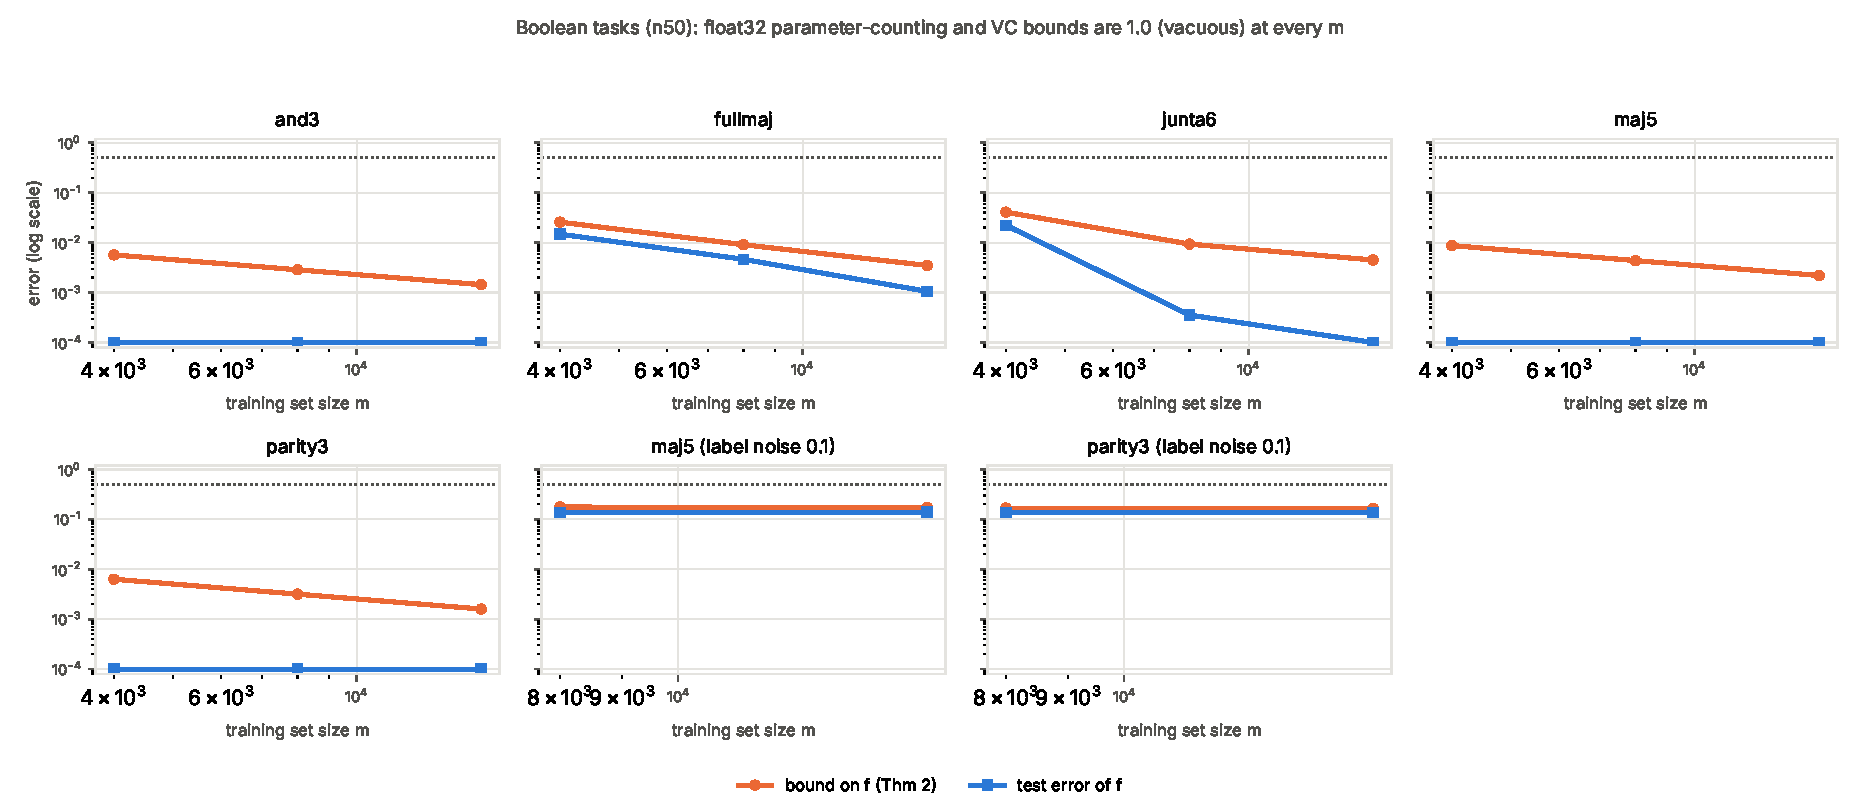
\includegraphics[width=\linewidth]{../figures/boolean_n50.pdf}
\caption{Boolean tasks, $n=50$: test error of the trained network $f$ (blue) and the certified upper bound on it from \cref{thm:reduction} (orange), averaged over 3 seeds, versus the number of training examples. The dotted line is chance.}\label{fig:boolean}
\end{figure}

\subsection{Distribution-free bounds by exact equivalence}\label{sec:exp-anyD}

With $n=20$ the whole input space has $2^{20}\approx10^6$ points, so the disagreement between $f$ and $g$ can be computed exactly, and \cref{cor:anyD} turns compression into a bound that holds for \emph{every} input distribution. \Cref{tab:boolean_n20} uses the same architecture and training protocol as before, with widths $(20,512,512,1)$. Once a network has learned its target (test error below $10^{-5}$), its compressed description agrees with it on all $2^{20}$ inputs, or on all but at most 8 of them. Appending the exception set $E$ then costs at most about 150 bits, and the distribution-free bound is close to the uniform-distribution bound: 0.0065 against 0.0061 for \texttt{parity3} at $m=4000$, 0.018 against 0.017 for \texttt{junta6}, and 0.024 against 0.008 for \texttt{fullmaj}, whose compressed descriptions disagree with $f$ on 2--6 inputs. When $f$ still errs on a small fraction of inputs (e.g.\ \texttt{maj5} at $m=250$, with 560--3700 exceptions), the uniform-distribution bound is non-vacuous (0.12) but the distribution-free one is not: listing the exceptions costs far more bits than 250 training points can pay for. Listing $E$ costs about $|E|\log_2(2^{20}e/|E|)$ bits (7{,}000--35{,}000 here), so \cref{cor:anyD} is informative only when that is small compared with $m$. This is a limitation of the exact-equivalence route, which has to describe $f$ exactly, not of distribution-free bounds as such. For one-hidden-layer networks, the dithered transfer theorem (\cref{sec:exp-t3}) gives distribution-free bounds without exact equivalence, by certifying $f$ only at the inputs where its margins allow.

\begin{table}[t]
\centering\small
\begin{tabular}{l r r r r r r}
\toprule
task & $m$ & test err.\ $f$ & bound on $f$ & bits of $g$ & any-$D$ bound & $|E|$ \\
\midrule
\texttt{fullmaj} & 4000 & 0.0000 & 0.0078 & 41 & 0.0236 & 5 \\
\addlinespace[2pt]
\texttt{junta6} & 100 & 0.3677 & 0.8149 & 22 & 1.0000 & 270461 \\
\texttt{junta6} & 4000 & 0.0000 & 0.0168 & 93 & 0.0184 & 0 \\
\addlinespace[2pt]
\texttt{maj5} & 100 & 0.0700 & 0.3870 & 51 & 1.0000 & 73405 \\
\texttt{maj5} & 250 & 0.0022 & 0.1225 & 42 & 1.0000 & 2257 \\
\texttt{maj5} & 500 & 0.0000 & 0.0621 & 42 & 0.1237 & 3 \\
\texttt{maj5} & 1000 & 0.0000 & 0.0315 & 42 & 0.0431 & 1 \\
\texttt{maj5} & 4000 & 0.0000 & 0.0080 & 42 & 0.0083 & 0 \\
\addlinespace[2pt]
\texttt{parity3} & 100 & 0.4933 & 0.9631 & 33 & 1.0000 & 300840 \\
\texttt{parity3} & 250 & 0.4507 & 0.9118 & 449 & 1.0000 & 255715 \\
\texttt{parity3} & 500 & 0.1834 & 0.2773 & 31 & 1.0000 & 190059 \\
\texttt{parity3} & 1000 & 0.0000 & 0.0242 & 31 & 0.0545 & 2 \\
\texttt{parity3} & 4000 & 0.0000 & 0.0061 & 31 & 0.0065 & 0 \\
\bottomrule
\end{tabular}
\caption{Boolean tasks, $n=20$: test error of the trained network $f$ (273,921 parameters) and the bound on it (\cref{thm:reduction}), averaged over 3 seeds; `bits' is the description length of the compressed $g$ (including the 4-bit design charge). The any-$D$ bound (\cref{cor:anyD}) holds for every input distribution; it patches $g$ on the set $E$ of inputs where $g\ne f$ (enumerated over all $2^{20}$ inputs). The parameter-counting and VC bounds for $f$ are 1.0 in every row.}\label{tab:boolean_n20}
\end{table}



\subsection{Images: bounds with unlabeled inputs}\label{sec:exp-t2}

With unlabeled inputs from $D_X$, \cref{thm:reduction} applies to image classifiers directly; this is the setting of \citet{bazinet2026bound}, and we include it to place the other results. The surrogate $g$ is the init-relative, DCT-coded, quantized network of \cref{sec:methods}, fine-tuned with a rate penalty using training labels, $f$'s outputs, or both. The disagreement is measured on the 10{,}000 test images without their labels, with a union bound over the $K$ compression configurations tried for each $f$. \Cref{tab:t2} reports the best Occam bound on $g$ itself and the best bound on $f$; each row is one trained network. On MNIST the bound on $f$ is 0.31 for 100 hidden units (test error 2.3\%, description 18k bits) and 0.37 for 256 (2.0\%, 28k bits); on Fashion-MNIST it is 0.53 and 0.62. Parameter-counting and VC bounds are 1.0 for all of these networks. The disagreement term adds 0.03--0.11 to the Occam bound on $g$. Most of the rest is the cost of the description: $g$'s training error is 2--14\%, and 17--29 thousand bits against $m=60000$ examples add another 0.24--0.39. Our compressor is simple and uses a data-independent prior, so these bounds are much weaker than those of \citet{bazinet2026bound}, who report 1.8--3.5\% for an MNIST CNN using surrogates trained on part of the training set: 1.8\% for a surrogate retrained on a random subset and tested on the remaining training examples, 3.5\% for a compressed surrogate with a data-dependent prior. Coding the first-layer update in the DCT basis instead of the pixel basis saves 22\% of the bits (18.4k against 23.5k; bound 0.31 against 0.37). Every network selected the largest rate penalty on the grid, so a wider grid would probably help.

\begin{table}[t]
\centering\small
\begin{adjustbox}{max width=\linewidth}\begin{tabular}{l l l r r r r r r r}
\toprule
data & network & basis & test err.\ $f$ & $K$ & bound on $g$ & bits & bound on $f$ & bits & $\Pr[f\ne g]$ \\
\midrule
fashion & 784-100-10 & dct & 0.1168 & 8 & 0.422 & 16594 & 0.532 & 16594 & 0.0997 \\
fashion & 784-256-10 & dct & 0.1106 & 8 & 0.512 & 28755 & 0.619 & 28755 & 0.0968 \\
mnist & 784-100-10 & dct & 0.0229 & 27 & 0.276 & 18371 & 0.313 & 18371 & 0.0302 \\
mnist & 784-100-10 & id & 0.0229 & 8 & 0.327 & 23522 & 0.370 & 23522 & 0.0352 \\
mnist & 784-256-10 & dct & 0.0197 & 27 & 0.339 & 27651 & 0.368 & 27651 & 0.0227 \\
\bottomrule
\end{tabular}\end{adjustbox}
\caption{Bounds with unlabeled inputs. `Bound on $g$': Occam bound (\cref{lem:occam}) for the best compressed network among $K$ configurations. `Bound on $f$': \cref{thm:reduction}, with $\Pr[f\ne g]$ estimated on the 10{,}000 test images without their labels, union-bounded over the $K$ configurations. Parameter-counting and VC bounds for $f$ are 1.0 in every row.}\label{tab:t2}
\end{table}



\subsection{Images and Boolean tasks: bounds from training data alone}\label{sec:exp-t3}

These are the bounds the question asks for in its strictest form: a deterministic bound on the error of the trained network itself, computed from the training set alone, with no validation data, no unlabeled data and no knowledge of the input distribution.

\paragraph{Worst-case weight sets (\cref{thm:certified}) are hopeless for dense networks.} On a 784--100--10 MNIST network (test error 2.4\%) we quantized the first-layer update in the DCT basis and certified with per-unit, per-band $\ell_2$ balls around the quantized network that contain $f$. At every step size the certified first-layer radius is 12--13 times the actual first-layer error $|Rx|$. Certifying 95\% of the training points needs steps of 2\% of the update's RMS, i.e.\ $6.1\times10^5$ bits for the first layer alone, ten times more than $m=6\times10^4$ (\repo{results/mnist/t3_worstcase_probe.txt}).

\paragraph{Dithered compression (\cref{thm:dither,lem:cert}).} \Cref{tab:t3} reports the bound for one-hidden-layer networks trained in the standard way (Adam, 20 epochs). It is non-vacuous (below the chance level of 0.9) for narrow networks: 0.44 for $H=8$ (test error 7.0\%) and 0.55 for $H=16$ (5.1\%) on MNIST, and 0.66 for $H=16$ on Fashion-MNIST. It degrades with width: 0.70 at $H=32$, 0.87 at $H=64$, 0.97 at $H=128$. Dithering does what it was designed to do. At comparable certified fractions it needs about 3 bits per first-layer coefficient instead of the 6--8 bits of worst-case sets (\repo{results/mnist/t3_worstcase_probe.txt}), because the certificate scales with the $\ell_2$ aggregate of the noise rather than its $\ell_1$ worst case. But at the measured 2.1--3.6 bits per first-layer coefficient (3.2--3.6 for $H\le32$), $784H$ coefficients exceed $m=6\times10^4$ bits once $H\gtrsim25$, and the total grows linearly in $H$.

Three ablations on the 32-unit network: coding the first layer in the pixel basis instead of the DCT basis costs 36\% more bits (bound 0.81 instead of 0.70); training with Gaussian weight noise of one or two times the initial RMS changes little (0.71, 0.69); a deterministic DCT initialization gives a more compressible network (67k instead of 84k bits; bound 0.69).

\paragraph{Networks with sparse updates.} The cost is driven by the number of first-layer coefficients that have to be described. Since exactly-zero coefficients are sent exactly (no dither, no noise, \cref{sec:methods}), a network whose update is sparse in the DCT basis is much cheaper. We trained 100- and 256-unit networks normally, kept the largest 0.1--3\% of the update's DCT coefficients and fine-tuned with that support fixed. Pruning followed by fine-tuning is a standard way to obtain small deployable networks \cite{zhou2019deconstructing}, and the bound is still on the network that was trained and deployed. \Cref{tab:t3sparse} shows the result. A standard-width MNIST network (100 hidden units) with 1\% of its update coefficients nonzero has test error 4.6\% and a training-data-only bound of 0.31. Keeping 0.3\% gives 7.2\% and 0.30, and 256-unit networks reach 0.40. The description is then 11--32 thousand bits. Each kept first-layer coefficient costs 5--8 bits for its value and 6--9 bits for its position, and the output layer takes 20--75\% of the total. For the output layer the search always picked the largest step multiplier on its grid, so a wider grid would probably help a little.

\begin{table}[t]
\centering\small
\begin{tabular}{l r l l r r r r r}
\toprule
data & $H$ & training & code & test err.\ $f$ & bits & certified & bound on $f$ & 32-bit Occam \\
\midrule
mnist & 32 & standard & DCT & 0.0323 & 84106 & 0.950 & 0.703 & 1.0 \\
mnist & 64 & standard & DCT & 0.0250 & 158075 & 0.966 & 0.871 & 1.0 \\
\bottomrule
\end{tabular}
\caption{Bounds on the original one-hidden-layer network $f$ from the 60{,}000 training examples alone (\cref{thm:dither,lem:cert}): no validation set and no unlabeled data. `Certified': fraction of training points with $\pi_g=1$. `Noise $\sigma$': $f$ trained with Gaussian weight noise of $\sigma$ times each tensor's initial RMS. Chance level is 0.9.}\label{tab:t3}
\end{table}


\begin{table}[t]
\centering\small
\begin{tabular}{l r r r r r r r}
\toprule
data & $H$ & kept coefficients & test err.\ $f$ & bits & certified & bound on $f$ & 32-bit Occam \\
\midrule
mnist & 100 & 3.0\% & 0.0333 & 32455 & 0.963 & 0.407 & 1.00 \\
mnist & 100 & 1.0\% & 0.0462 & 17664 & 0.945 & 0.314 & 1.00 \\
mnist & 100 & 0.3\% & 0.0722 & 11423 & 0.909 & 0.304 & 1.00 \\
mnist & 256 & 0.3\% & 0.0441 & 23244 & 0.924 & 0.399 & 1.00 \\
mnist & 256 & 0.1\% & 0.0647 & 21673 & 0.916 & 0.398 & 1.00 \\
fashion & 100 & 1.0\% & 0.1693 & 20176 & 0.828 & 0.501 & 1.00 \\
fashion & 100 & 0.3\% & 0.1926 & 13170 & 0.798 & 0.468 & 1.00 \\
\bottomrule
\end{tabular}
\caption{As \cref{tab:t3}, for networks whose first-layer update is exactly sparse in the DCT basis (trained, pruned to the stated fraction of coefficients, fine-tuned with the support fixed). The support is part of the description; only nonzero coefficients are dithered.}\label{tab:t3sparse}
\end{table}


\paragraph{Boolean networks: a bound for every input distribution.} \Cref{tab:boolean_t3} applies the same theorem to one-hidden-layer networks on Boolean tasks. Since it uses only the training sample, the bound holds whatever distribution generated the inputs. The bounds are 0.06--0.33 for networks with 16 or 32 hidden units at $m=16000$ (0.23 at $m=4000$). With the uniform distribution known, \cref{thm:reduction} on the same networks is 30--150 times tighter (0.0015--0.007), which measures what knowledge of the input distribution buys.

\begin{table}[t]
\centering\small
\begin{tabular}{l r r r r r r r r}
\toprule
task & $n$ & $m$ & $H$ & test err.\ $f$ & bits & training-data-only bound & bits & known-$D_X$ bound \\
\midrule
\texttt{maj5} & 20 & 4000 & 16 & 0.0000 & 1529 & 0.234 & 38 & 0.007 \\
\texttt{maj5} & 20 & 16000 & 16 & 0.0000 & 1523 & 0.064 & 38 & 0.002 \\
\texttt{parity3} & 20 & 16000 & 16 & 0.0000 & 2009 & 0.084 & 31 & 0.002 \\
\texttt{and3} & 50 & 16000 & 16 & 0.0000 & 3791 & 0.152 & 32 & 0.002 \\
\texttt{fullmaj} & 50 & 16000 & 16 & 0.0000 & 3629 & 0.151 & 48 & 0.002 \\
\texttt{junta6} & 50 & 16000 & 32 & 0.0000 & 9132 & 0.327 & 102 & 0.005 \\
\texttt{maj5} & 50 & 16000 & 16 & 0.0000 & 2589 & 0.110 & 45 & 0.002 \\
\texttt{maj5}, noise 1 & 50 & 16000 & 16 & 0.0000 & 2331 & 0.099 & 45 & 0.002 \\
\texttt{maj5} & 50 & 16000 & 32 & 0.0000 & 5468 & 0.213 & 45 & 0.002 \\
\texttt{parity3} & 50 & 16000 & 32 & 0.0000 & 7113 & 0.266 & 35 & 0.002 \\
\bottomrule
\end{tabular}
\caption{Boolean tasks, one-hidden-layer networks: the training-data-only bound (\cref{thm:dither}), which holds whatever the input distribution, against the bound that uses the known uniform input distribution (\cref{thm:reduction}) on the same network.}\label{tab:boolean_t3}
\end{table}



\subsection{Initialization}\label{sec:exp-init}

\paragraph{Coding relative to the initialization.} \Cref{tab:init} trains the same 784--256--10 network from three initialization scales and from a deterministic DCT initialization, and codes the update either relative to the (free) initialization or relative to zero, with the unlabeled-data codec of \cref{sec:exp-t2}. \Cref{tab:t3} makes the same comparison for the dithered training-data-only code of a 32-unit network: coding relative to zero costs 84{,}269 bits against 83{,}976, a difference of 0.3\%. Two effects explain why the initialization matters so little here. First, Adam moves the first-layer weights far from their initial values, so the update is not small compared with the initialization. Second, in the dithered code the steps in the high-frequency DCT bands are coarse, because natural images have little energy there, so describing the random initial weights in those bands costs almost nothing. The deterministic DCT initialization, which costs nothing either, led to a more compressible network: 67k bits against 84k.

\begin{table}[t]
\centering\small
\begin{tabular}{l r l r r r r r}
\toprule
initialization & scale & code relative to & test err.\ $f$ & bound on $g$ & bits & bound on $f$ & bits \\
\midrule
seeded random & 0.3 & initialization & 0.0199 & 0.384 & 34421 & 0.407 & 34421 \\
seeded random & 1 & initialization & 0.0197 & 0.367 & 32264 & 0.391 & 32264 \\
seeded random & 1 & zero & 0.0197 & 0.377 & 34095 & 0.399 & 34095 \\
\bottomrule
\end{tabular}
\caption{MNIST, 784-256-10: description length and bounds when the update is coded relative to the (free) initialization or relative to zero, for three initialization scales and a deterministic initialization. Best of 8 compression configurations each.}\label{tab:init}
\end{table}


\paragraph{The init-kernel codec in the lazy and rich regimes.} \Cref{tab:kernel} compares, on the same Boolean networks ($n=30$, one hidden layer of 512 units), the init-kernel codec of \cref{prop:kernel} with function-space distillation. The lazy regime uses initialization scale 2 and plain SGD; the parameters then move by about 10\% of their initial norm, and $f$ agrees with its linearization at $\theta_0$ on 97--99.9\% of inputs. The rich regime uses scale 0.1 and Adam; the parameters move by 3--5 times their initial norm and the linearization is poor. The init-kernel codec describes $\theta_0+P_r\Delta$, where $P_r$ projects onto the top-$r$ eigenvectors of the uniform-input empirical kernel at $\theta_0$. That kernel is estimated from 4000 uniform inputs, so it is free given $\theta_0$. The candidate ranks include the dimensions of the low-degree Walsh spaces: $1+n=31$, $1+n+\binom n2=466$ and $4526$.

The results match the picture of \cref{sec:init-theory}.
\begin{itemize}
\item In the lazy regime the best rank is the dimension of the low-degree Walsh space that the target lives in. For the majority targets it is exactly $r=31$, the dimension of the functions of degree at most 1, and the bounds are 0.05--0.25. For the degree-2 target \texttt{parity2} it is exactly $r=466$, the dimension of degree at most 2. Describing 466 coefficients costs about 1500 bits, so the bound is still 0.59 at $m=4000$; the distilled junta needs 20 bits and gets 0.006. The estimated bound as a function of $r$ has a sharp minimum at these dimensions (\cref{fig:kernel}). This is the $n^k$ sample complexity of kernel methods appearing as description length.
\item In the rich regime the update is far from the initial kernel's top eigenspace and the codec fails.
\item Function-space distillation does better in both regimes. It describes the function, not the update, so how far training moved from the initialization does not matter to it.
\end{itemize}

\begin{table}[t]
\centering\small
\begin{adjustbox}{max width=\linewidth}\begin{tabular}{l l r r r r r r r r}
\toprule
task & regime & $m$ & test err.\ $f$ & move & lin.\ dis. & $r$ & bits & init-kernel bound & distillation bound \\
\midrule
\texttt{fullmaj} & lazy & 1000 & 0.0387 & 0.11 & 0.015 & 31 & 205 & 0.253 & 0.080 \\
\texttt{fullmaj} & rich & 1000 & 0.0000 & 4.57 & 0.346 & 16 & 124 & 0.821 & 0.036 \\
\texttt{fullmaj} & lazy & 4000 & 0.0039 & 0.17 & 0.032 & 31 & 241 & 0.143 & 0.013 \\
\texttt{fullmaj} & rich & 4000 & 0.0000 & 4.71 & 0.277 & 31 & 196 & 0.502 & 0.009 \\
\texttt{maj5} & lazy & 1000 & 0.0010 & 0.09 & 0.002 & 31 & 208 & 0.158 & 0.033 \\
\texttt{maj5} & rich & 1000 & 0.0000 & 3.32 & 0.080 & 31 & 170 & 0.288 & 0.032 \\
\texttt{maj5} & lazy & 4000 & 0.0003 & 0.09 & 0.001 & 31 & 214 & 0.052 & 0.009 \\
\texttt{maj5} & rich & 4000 & 0.0000 & 3.98 & 0.197 & 31 & 213 & 0.297 & 0.008 \\
\texttt{parity2} & lazy & 1000 & 0.0181 & 0.17 & 0.168 & 466 & 1519 & 0.940 & 0.039 \\
\texttt{parity2} & rich & 1000 & 0.0000 & 3.58 & 0.434 & 2048 & 8230 & 1.000 & 0.020 \\
\texttt{parity2} & lazy & 4000 & 0.0003 & 0.18 & 0.133 & 466 & 1524 & 0.591 & 0.006 \\
\texttt{parity2} & rich & 4000 & 0.0000 & 3.53 & 0.410 & 2048 & 6094 & 0.772 & 0.005 \\
\bottomrule
\end{tabular}\end{adjustbox}
\caption{Boolean tasks ($n=30$, one hidden layer of 512): the init-kernel codec of \cref{prop:kernel} ($\theta_0$ plus the top-$r$ eigenvectors of the uniform-input empirical NTK at $\theta_0$, both free) against function-space distillation, on the same networks. `Move': $\|\theta-\theta_0\|/\|\theta_0\|$; `lin.\ dis.': disagreement between $f$ and its linearization at $\theta_0$. One seed per row.}\label{tab:kernel}
\end{table}


\begin{figure}[t]
\centering
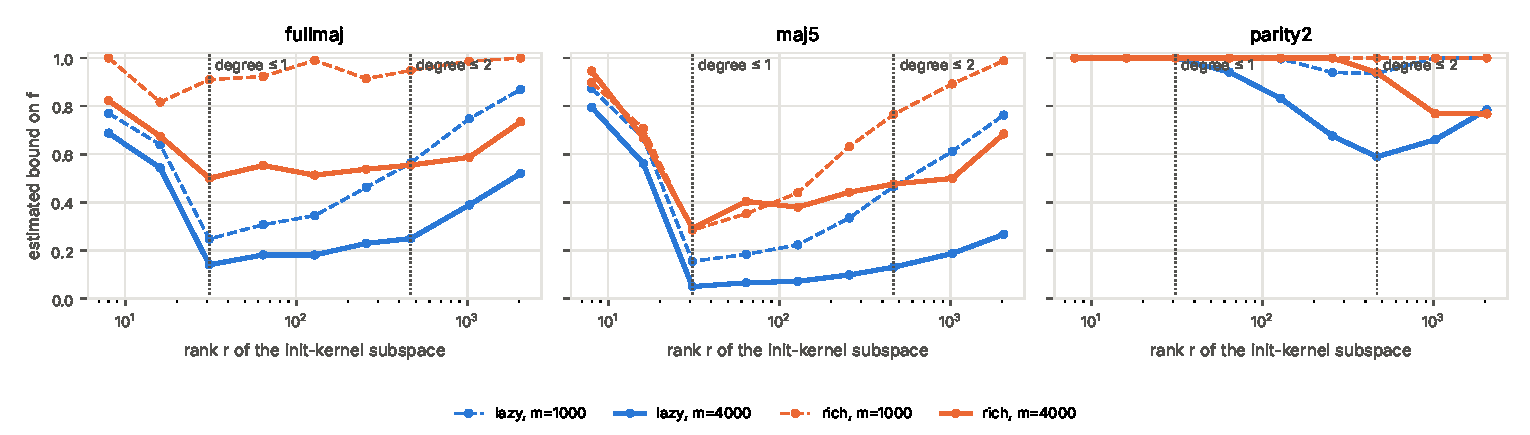
\includegraphics[width=\linewidth]{../figures/init_kernel.pdf}
\caption{Init-kernel codec: estimated bound on $f$ (Occam term plus disagreement on a selection pool) as a function of the rank $r$ of the subspace spanned by the top eigenvectors of the initial kernel, for networks trained in the lazy (blue) and rich (orange) regimes. Dotted lines: dimensions of the Walsh spaces of degree at most 1 ($1+n$) and at most 2 ($1+n+\binom n2$).}\label{fig:kernel}
\end{figure}

